\section{\gls{mtbusb} v4}

\begin{figure}[ht]
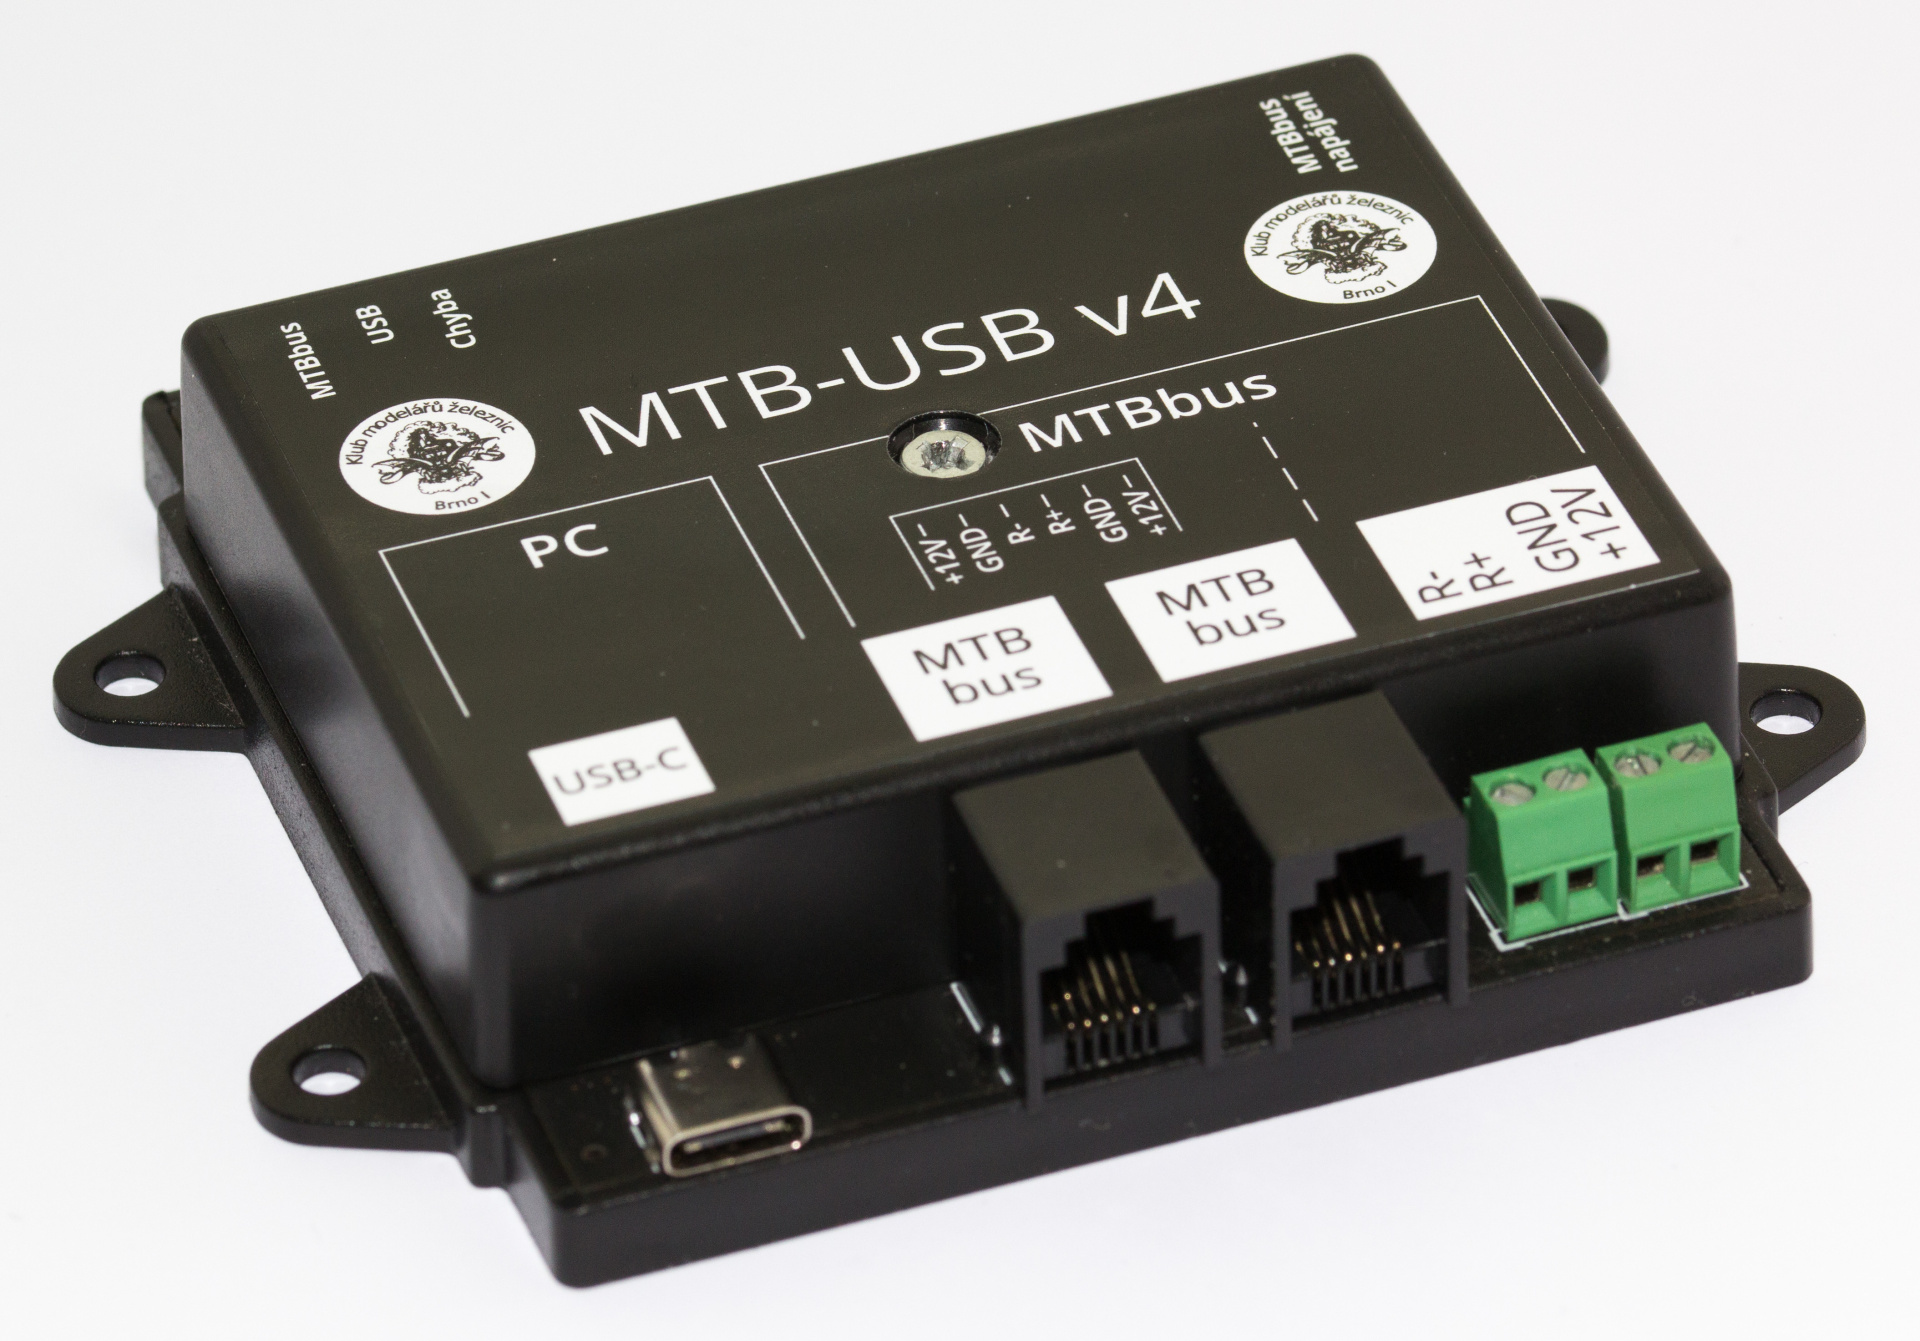
\includegraphics[width=0.7\textwidth]{data/usb-all.jpg}
\caption{Prototyp modulu MTB-USB.}
\label{fig:mtbusb-prototype}
\end{figure}

\gls{mtbusb} modul vzniknuvší v~rámci této práce byl navržen od základu znovu,
inspirace současným \gls{mtbusb} modulem je minimální. Vznikly hardware,
firmware a~popisy komunikačních protokolů.

Hlavním úkolem \gls{mtbusb} modulu je přeposílat data mezi sběrnici \gls{mtbbus}
a~počítačem. \gls{mtbusb} provádí časově kritické operace sběrnice – například
počítání timeoutu odpovědi na zprávu od \gls{mtb} modulů nebo pravidelné
dotazování \gls{mtb} modulů. Počítač je o~dění na \gls{mtbbus} informován
formou událostí.

\subsection{Komunikační protokol s~počítačem}

Před implementací \gls{mtbusb} modulu je třeba navrhnout komunikační protokol
s~počítačem. Tento komunikační protokol musí být přirozeně jiný, než nový
komunikační protokol sběrnice \gls{mtbbus}, který jsme popsali v~předchozí
kapitole, protože zahrnuje jiné aktéry a~funguje na jiném hardwaru.

Komunikační protokol \gls{mtbusb} a~počítače je navržen tak, aby byl do velké
míry nezávislý na protokolu sběrnice \gls{mtbbus}. Nejdůležitější zprávou mezi
počítačem a~\gls{mtbusb} je požadavek o~přeposlání zprávy mezi \gls{usb}
a~\gls{mtbbus}. Tato zpráva umožňuje počítačovému programu poslat libovolnou
zprávu libovolnému \gls{mtb} modulu (a~naopak), aniž by \gls{mtbusb} deska
musela znát sémantiku této zprávy. Protokol sběrnice \gls{mtbbus} byl
vytvářen přesně s~tímto cílem.

Na \gls{mtbusb} desku můžeme tedy pohlížet v~zásadě jako na tenkého
přeposílatele mezi dvěma různými sběrnicemi – tzv. \textit{gateway}.

Plnohodnotná specifikace protokolu mezi počítačem a \gls{mtbusb} je
k~dispozici na \url{https://github.com/kmzbrnoI/mtbbus-protocol/tree/master/pc}.
Popišme nyní stručně návrh protokolu.

Mezi počítačem a \gls{mtbusb} deskou se komunikuje po virtuálním sériovém portu
(tzv. \textit{\gls{cdc}}) tunelovaným skrze \gls{usb} rozhraní. Toto řešení
bylo vybráno, protože je prakticky standardem pro připojení speciálních
periferií k~počítači.  Zvažován byl také například \textit{\gls{hid}}.
\gls{usb} nezná pojem zprávy tak, jak bychom
vyžadovali\footnote{Při užití třídy \gls{cdc} se data posílají nejčastěji
každou milisekundu a to v~bloku o~nejvýše 64 bytech.  Počítačová aplikace díky
bufferování operačního systému není schopna tyto bloky spolehlivě rozlišit.}.
Protože USB podporuje pouze 8bitový sériový port, začátek zprávy je třeba
označit jiným způsobem než pomocí 9. bitu. V~navrženém protokolu je začátek
zprávy označen speciální sekvencí dvou bytů \texttt{0x2A} a \texttt{0x42}. Tato sekvence
se sice ve zprávě může objevit, ale pravděpodobnost, že dojde k~tolika chybám,
aby tato sekvence uprostřed zprávy byla považována za začátek zprávy, je
malá.\footnote{Rozdělování dat do zpráv na straně přijímače se
nemusí řídit jen detekcí sekvence \texttt{0x2A 0x42}. Pokud zprávy nechodí moc
často, lze po delší době nepřijímání dat (řádově jednotky milisekund) vyprázdnit
vstupní buffer a~očekávat tedy, že další příchozí data budou novou zprávou.
Odesílatel zprávy nesmí posílat jednotlivé části zprávy s~velkou prodlevou, to
je ale splnitelný požadavek.}

Každá zpráva mezi počítačem a \gls{mtbusb} má následující strukturu.

\begin{compactenum}
\item \texttt{0x2A},
\item \texttt{0x42},
\item počet následujících bytů,
\item kód zprávy,
\item data zprávy (až 122 bytů).
\end{compactenum}

Struktura je podobná struktuře zprávy protokolu \gls{mtbbus}, viz
\ref{subsub:mtbbus-proto-strucure}. Zpráva neobsahuje kontrolní součet, protože
integritu zprávy řeší přímo \gls{usb}.
Upozorňujeme, že \textit{kód zprávy} není kód zprávy \gls{mtbbus},
ale kód zprávy protokolu PC – \gls{mtbusb}.

Zprávy z~počítače pro \gls{mtbusb} jsou:

\begin{itemize}
\item \textbf{Forward packet to \gls{mtbbus}}

V~\textit{datech zprávy} následují adresa a~zpráva pro \gls{mtb} modul.

\item \textbf{MTB-USB Information Request}

\item \textbf{Change Speed}

Požadavek na změnu komunikační rychlosti \gls{mtbusb} modulu. Změnu rychlosti
jednotlivých \gls{mtb} modulů je třeba provést předchozím příkazem, typicky
broadcastem všem \gls{mtb} modulům.

\item \textbf{Active modules request}

Odpovědí na tento příkaz je seznam aktivních \gls{mtb} modulů.

\end{itemize}

Zprávy z~\gls{mtbusb} pro počítač jsou:

\begin{itemize}
\item \textbf{Acknowledgement}
\item \textbf{Error}
\item \textbf{Packet from \gls{mtbbus}}

Zpráva je odeslána počítači při odpovědi \gls{mtb} modulu na zprávu z~počítače
nebo na pravidelný sken \gls{mtb} modulů. Z~pohledu počítače tak přichází jak
odpovědi na příkazy pro \gls{mtb} modul, které poslal počítač, tak asynchronní
události – například informace o~změně stavu vstupů.

\item \textbf{\gls{mtbusb} Information}

\item \textbf{Active modules list}

\item \textbf{New module discovered event}

\item \textbf{Module failed event}

\end{itemize}

\gls{mtbusb} si udržuje seznam aktivních \gls{mtb} modulů. Polling
modulů probíhá v~iteracích. V~každé iteraci jsou osloveny všechny aktivní
moduly a 10 neaktivních modulů. Tím je zaručeno, že aktivní moduly jsou
skenovány často a~zároveň jsou detekovány moduly nové.

Pokud \gls{mtb} modul neodpoví na \textit{Module Inquiry}
(\ref{subsub:mtbbus-messages}), počítači je odeslána zpráva \textit{Module
failed event}. Modul je považován za ztracený, jakmile neodpoví na
\textit{Module Inquiry} ve třech po sobě jdoucích iteracích. Zpráva
\textit{Module failed event} je při úplném výpadku modulu odeslána
celkem třikrát proto, aby bylo možné z~počítače monitorovat chod sběrnice.
Občasné neodpovídání modulů na výzvy je dobrým indikátorem problémů sběrnice.

Vlastností \gls{mtbbus} je, že každý \gls{mtb} modul musí vždy
odpovědět na každou zprávu, kterou dostane\footnote{Výjimkou jsou pouze
\textit{broadcast} zprávy.}. Protože \gls{mtbbus} je potenciálně nespolehlivé
médium, na kterém integritu příkazů kontrolujeme vlastními mechanismy, provádí
modul \gls{mtbusb} retransmisi zpráv \gls{mtb} modulům v~případě, že na zprávu
nepřijde žádná odpověď, a~to až třikrát. Proto je součástí zprávy \textit{Packet
from \gls{mtbbus}} také počítadlo, které říká, na kolikátý pokus byla
odpověď přijata (u~asynchronních událostí $0$). Toto číslo bylo do protokolu
vloženo opět se záměrem, aby bylo možné v~počítači monitorovat chod sběrnice.

Na dalších příkazech protokolu není vcelku nic zajímavého, pokud je čtenář chce
prostudovat, je mu k~dispozici plná specifikace protokolu\footnote{
\url{https://github.com/kmzbrnoI/mtbbus-protocol/tree/master/pc}}.

\subsection{Hardware} \label{subsec:mtbusb:hardware}

\begin{figure}[ht]
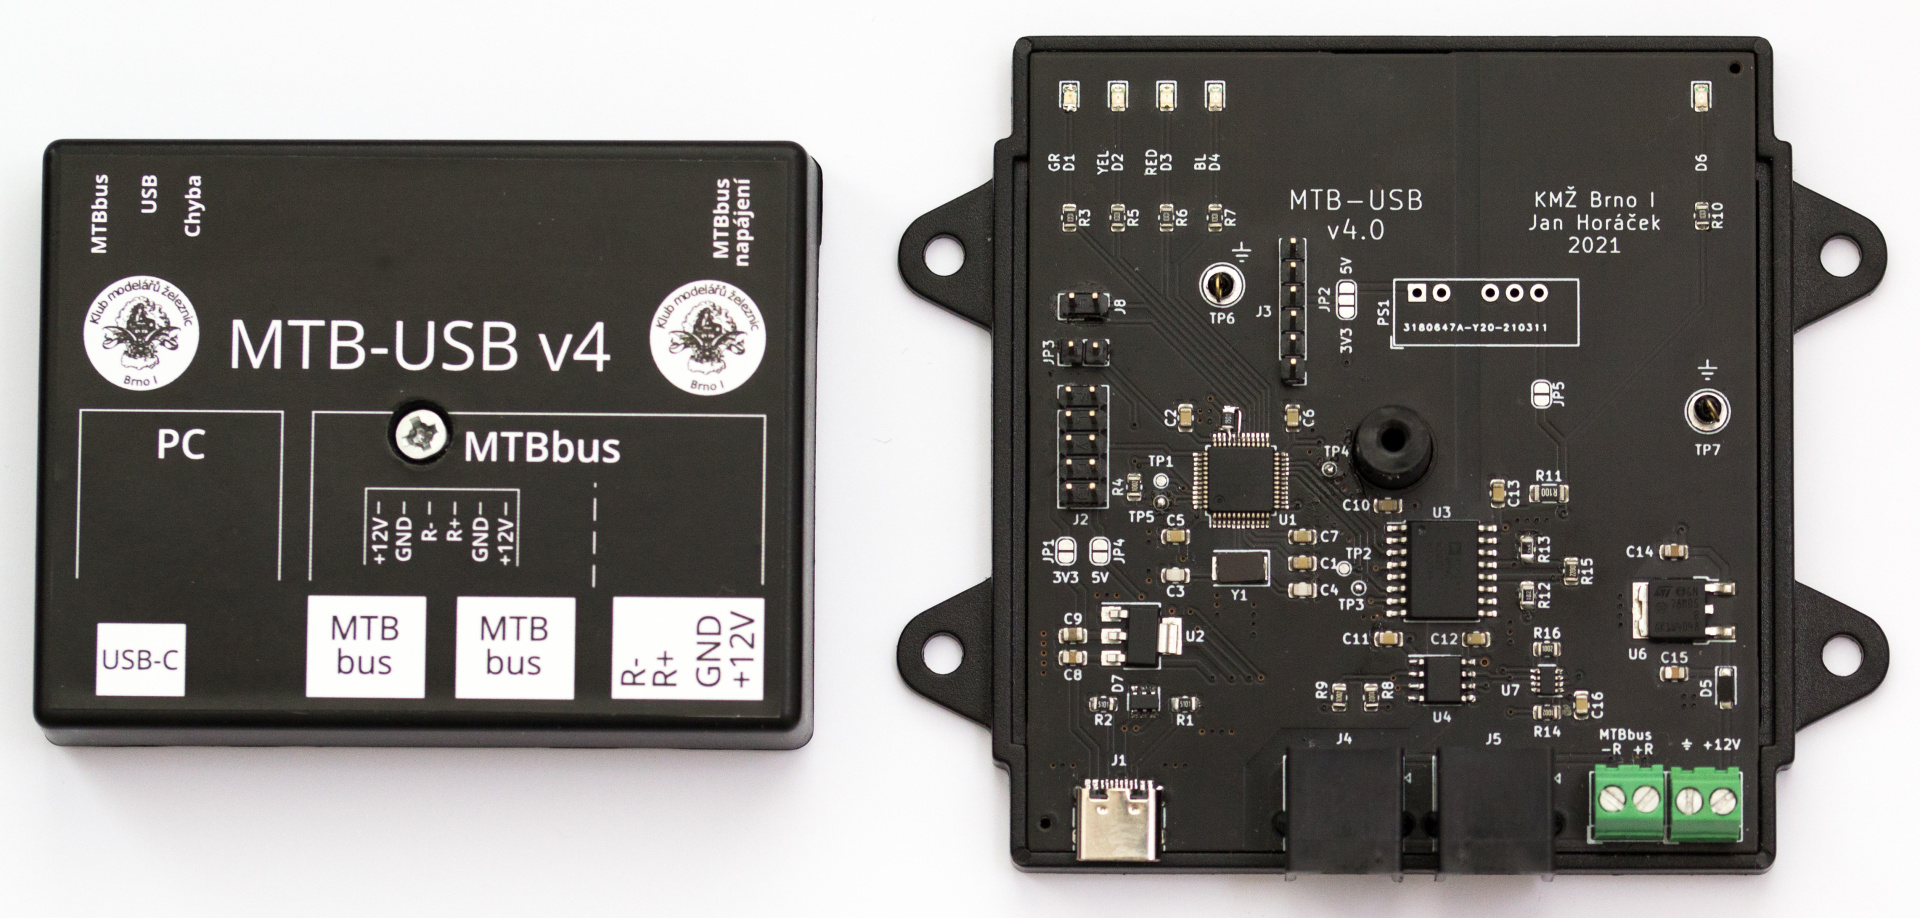
\includegraphics[width=\textwidth]{data/usb-inside.jpg}
\caption{Krabička a deska plošných spojů \gls{mtbusb}.}
\label{fig:mtbusb-inside}
\end{figure}

Srdcem \gls{mtbusb} modulu je procesor \texttt{STM32F103}, což je moderní
mikrokontrolér architektury \textit{ARM}. Autor jej zvolil z~několika důvodů.

\begin{compactenum}
\item Procesor \texttt{STM32F103} má hardwarovou podporu \gls{usb}.
\item Procesory \texttt{STM32} nabízí velké velikosti pamětí a výpočetní výkon.
\item Procesory \texttt{STM32} se stávají standardy v~embedded systémech.
\item Procesory \texttt{STM32} se dají velice snadno debugovat.
\item Procesor \texttt{STM32F103} je jako jeden z~mála \texttt{STM} součástí
	\textit{basic} součástek na \url{https://jlcpcb.com/}.
\item Autor se chtěl naučit pracovat s~novou architekturou procesorů.
\end{compactenum}

Hardwarová podpora \gls{usb} umožňuje výrazně vyšší flexibilitu komunikace
s~počítačem než použití historicky zaužívaných převodních obvodů mezi
\gls{usb} a~sériovou linkou. V~programu procesoru je tak například
možné definovat, že procesor má více \gls{cdc} linek – druhá se využije například
pro ladění programu. Procesor může v~budoucnu používat libovolnou třídu
\gls{usb}. Celé řešení se tak stává mnohem lépe upravitelné pouze změnou
softwaru, což je méně pracné, než změna hardwaru.

Všechny desky plošných spojů (\textit{\gls{dps}}) navržené v~rámci této práce
jsou vytvořeny tak, aby se daly automaticky osazovat na
JLCPCB\footnote{Aktuálně lze osazovat pouze jednu stranu
desky a pouze \textit{SMD} součástky.}. Tato firma nabízí automatické osazování
malých sérií \gls{dps} za dostupnou cenu, což výrazně zjednodušuje výrobu nových
komponent. \textit{JLCPCB} rozlišuje tzv. \textit{basic} a~\textit{extended}
součástky k~osazení, přičemž za \textit{basic} se neplatí režijní poplatek při
osazování. \textit{Basic} součástky jsou ty, které se používají skutečně často
(typicky diskrétní součástky – rezistory, kondenzátory apod.) a~u~kterých se
očekává, že se budou vyrábět i~za desítky let. Procesor \texttt{STM32F103} byl
zvolen mj. proto, že je \textit{basic} součástkou.

Schéma a výkres desky plošných spojů byly vytvořeny v~nástroji \textit{KiCad},
který autor této práce používal poprvé. Jedním z~hlavních přínosů celé této
práce pro něj je, že se naučil pracovat s~programem \textit{KiCad}. Schéma
a~výkres desky plošných spojů jsou k~dispozici
online\footnote{\url{https://github.com/kmzbrnoI/mtb-usb-4-pcb}}, schéma je
přiloženo také jako příloha této práce (\ref{fig:mtb-usb-sch}).

Popišme nyní stručné schéma. Schéma je na první pohled rozděleno na 2~části,
které jsou na desce plošných spojů (\textit{\gls{dps}}) galvanicky oddělené –
\gls{usb} část (vlevo) a~\gls{mtbbus} část (vpravo). \gls{usb} část obsahuje
procesor a je napájena přímo z~\gls{usb}. \gls{mtbbus} část obsahuje rozhraní
sběrnice \gls{mtbbus} a je napájena buď z~externího zdroje (ze stejného jako
zbytek sběrnice \gls{mtbbus}), nebo přes galvanicky oddělený měnič \texttt{PS1}.
Osazením nebo neosazením součástek se zvolí, která varianta se bude používat.

Hlavním prvkem \gls{usb} části schématu je již zmíněný procesor
\texttt{STM32F103} (vlevo nahoře). K~procesoru jsou připojena diagnostická
rozhraní (\texttt{J2}, \texttt{J3}). Celá \gls{usb} část je napájena z~\gls{usb}
portu, přičemž je využito moderního konektoru \gls{usb}-C.

Rozhraní \gls{usb} a \gls{mtbbus} části schématu tvoří galvanicky oddělený
budič sběrnice RS485 typu \texttt{ADM2483}. \texttt{ADM2483} je osvědčený budič,
který zvládá proudy sběrnice až do $250~mA$ \cite{adm2483-datasheet} a je tedy
vhodný pro komunikaci s~větším počtem \gls{mtb} modulů.

Specialitou \gls{mtbusb} modulu je měřící obvod \texttt{INA219} ve sběrnicové
části desky, který měří napětí a~proud do sběrnicové části obvodu
\texttt{ADM2483} a~posílá naměřenou hodnotu přes galvanický oddělovač do
procesoru. Procesor je tak schopen detekovat nestandardní chování sběrnice,
například zkrat.\footnote{Pro měření zatím není podpora v~komunikačním
protokolu s~počítačem a~ve firmwaru. Hardware je odzkoušený. Podporu je v~plánu
doplnit v~další verzi.}

Při návrhu desky plošných spojů bylo třeba vyřešit především to, do jaké
krabičky desku vložit. \gls{mtbusb} modul totiž typicky není pevnou součástí
kolejiště, je umístěn vedle kolejiště u~řídicího serveru. Vyvstal tak požadavek
modul zavřít do krabičky, ideálně s~možností uchycení na zeď. Po rešerši byla
zvolena krabička firmy \textit{Digikeijs}, jejíž zásadní výhodou je, že pro
vyvedení konektorů a indikačních LED není třeba do krabičky frézovat. Navíc lze
na krabičku velice elegantně nalepit potisk, který vysvětluje použití
jednotlivých konektorů a~význam LED. Celé řešení je zobrazeno na
obrázku \ref{fig:mtbusb-prototype}.


\subsection{Firmware}

Firmware je psaný v~jazyce \texttt{C}, který byl zvolen především proto, že ve
stejném jazyce je psána základní knihovna pro interakci s~periferiemi procesoru
\textit{STM32 HAL} \cite{stm32-hal}, kterou firmware využívá.

Při práci s~periferiemi je využito \textit{Direct Memory Access (DMA)}. Pro
komunikaci přes \gls{usb} byla využita komunitní knihovna
\texttt{libusb\_stm32}\footnote{\url{https://github.com/dmitrystu/libusb_stm32}}.

Celý firmware je k~dispozici pod opensource licencí
online\footnote{\url{https://github.com/kmzbrnoI/mtb-usb-4-fw}}.
